% This file was converted to LaTeX by Writer2LaTeX ver. 1.0.2
% see http://writer2latex.sourceforge.net for more info
\documentclass[a4paper]{article}
\usepackage[ascii]{inputenc}
\usepackage[T1]{fontenc}
\usepackage[spanish]{babel}
\usepackage{amsmath}
\usepackage{amssymb,amsfonts,textcomp}
\usepackage{color}
\usepackage{array}
\usepackage{hhline}
\usepackage{hyperref}
\hypersetup{pdftex, colorlinks=true, linkcolor=blue, citecolor=blue, filecolor=blue, urlcolor=blue, pdftitle=, pdfauthor=johanna , pdfsubject=, pdfkeywords=}
\usepackage[pdftex]{graphicx}
% Text styles
\newcommand\textstyleFuentedeprrafopredeter[1]{#1}
% List styles
\newcounter{saveenum}
\newcommand\liststyleLi{%
\renewcommand\theenumi{\arabic{enumi}}
\renewcommand\theenumii{\alph{enumii}}
\renewcommand\theenumiii{\roman{enumiii}}
\renewcommand\theenumiv{\arabic{enumiv}}
\renewcommand\labelenumi{\theenumi.}
\renewcommand\labelenumii{\theenumii.}
\renewcommand\labelenumiii{\theenumiii.}
\renewcommand\labelenumiv{\theenumiv.}
}
% Page layout (geometry)
\setlength\voffset{-1in}
\setlength\hoffset{-1in}
\setlength\topmargin{2cm}
\setlength\oddsidemargin{2cm}
\setlength\textheight{25.7cm}
\setlength\textwidth{17.001cm}
\setlength\footskip{0.0cm}
\setlength\headheight{0cm}
\setlength\headsep{0cm}
% Footnote rule
\setlength{\skip\footins}{0.119cm}
\renewcommand\footnoterule{\vspace*{-0.018cm}\setlength\leftskip{0pt}\setlength\rightskip{0pt plus 1fil}\noindent\textcolor{black}{\rule{0.25\columnwidth}{0.018cm}}\vspace*{0.101cm}}
% Pages styles
\makeatletter
\newcommand\ps@MP{
  \renewcommand\@oddhead{}
  \renewcommand\@evenhead{}
  \renewcommand\@oddfoot{}
  \renewcommand\@evenfoot{}
  \renewcommand\thepage{\arabic{page}}
}
\newcommand\ps@Standard{
  \renewcommand\@oddhead{}
  \renewcommand\@evenhead{}
  \renewcommand\@oddfoot{}
  \renewcommand\@evenfoot{}
  \renewcommand\thepage{\arabic{page}}
}
\makeatother
\pagestyle{Standard}
\title{}
\author{johanna }
\date{2015-11-16T09:35:55.320384018}
\begin{document}
\clearpage\clearpage\setcounter{page}{1}\pagestyle{MP}
{\centering\sffamily\bfseries
Instalaci\'on y Funcionalidad
\par}

\liststyleLi
\begin{enumerate}
\item \textstyleFuentedeprrafopredeter{\textsf{Crear una cuenta en
}}\url{https://github.com/}
\item {\sffamily
Validar la Cuenta en su correo para poder acceder e instalar nuevos
repositorios.}
\end{enumerate}


\begin{center}
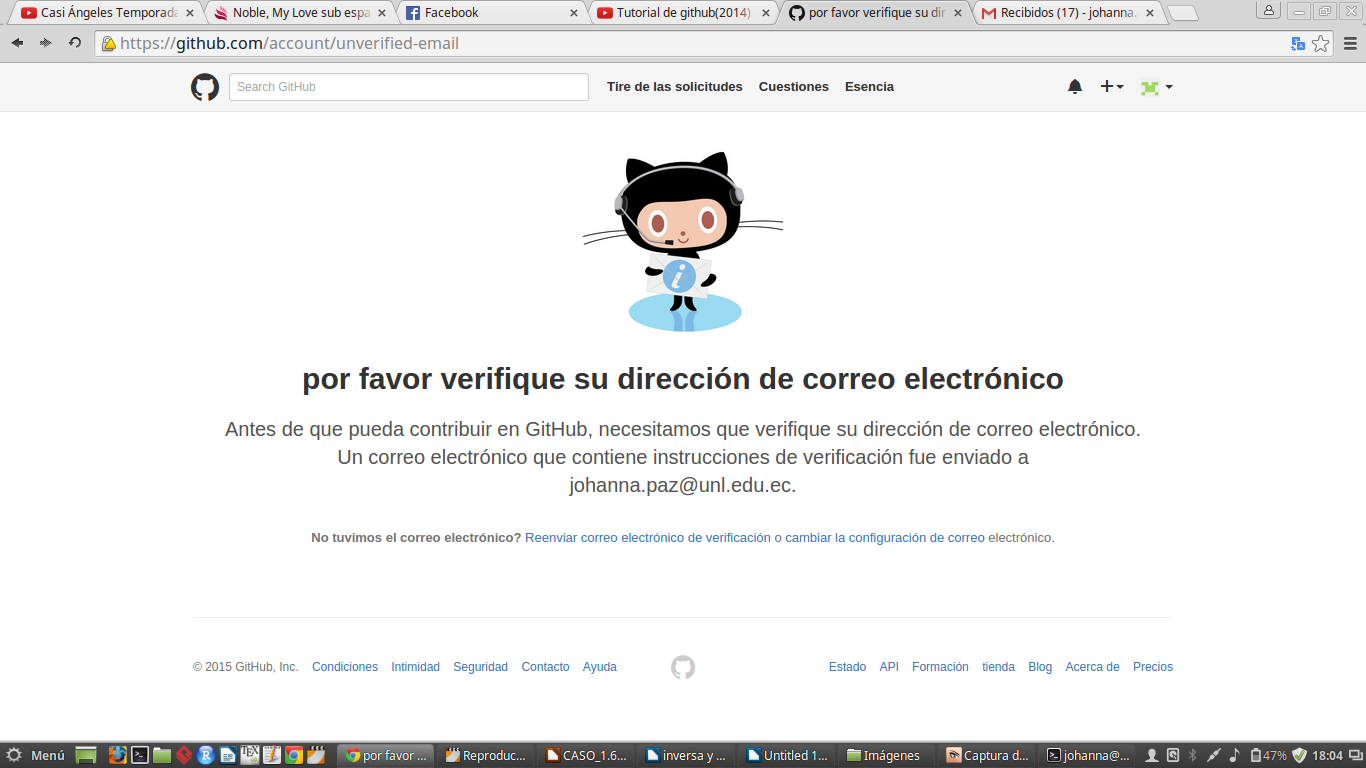
\includegraphics[width=17cm,height=9.557cm]{manual-img1.png}
\end{center}

\bigskip



\begin{center}
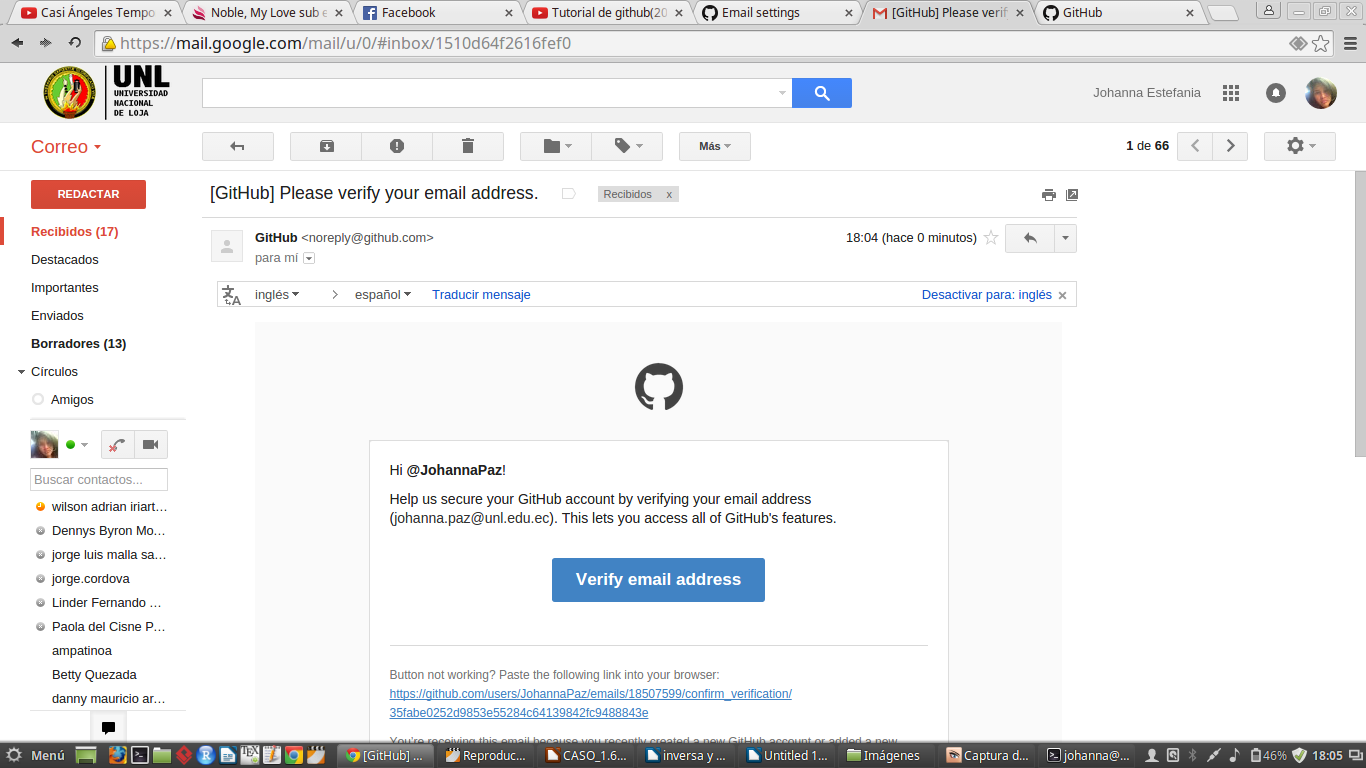
\includegraphics[width=17cm,height=9.557cm]{manual-img2.png}
\end{center}
{\sffamily
Ahora vamos \ a instalar Gihtub}

{\sffamily
Abrimos una terminal para ejecutar el siguiente comando:}

{\sffamily
\ \ \ \ sudo apt-get install git-core}

\liststyleLi
\setcounter{saveenum}{\value{enumi}}
\begin{enumerate}
\setcounter{enumi}{\value{saveenum}}
\item {\sffamily
Crear o ingresar en la carpeta q queremos clonar el repositorio}
\end{enumerate}

\bigskip



\begin{center}
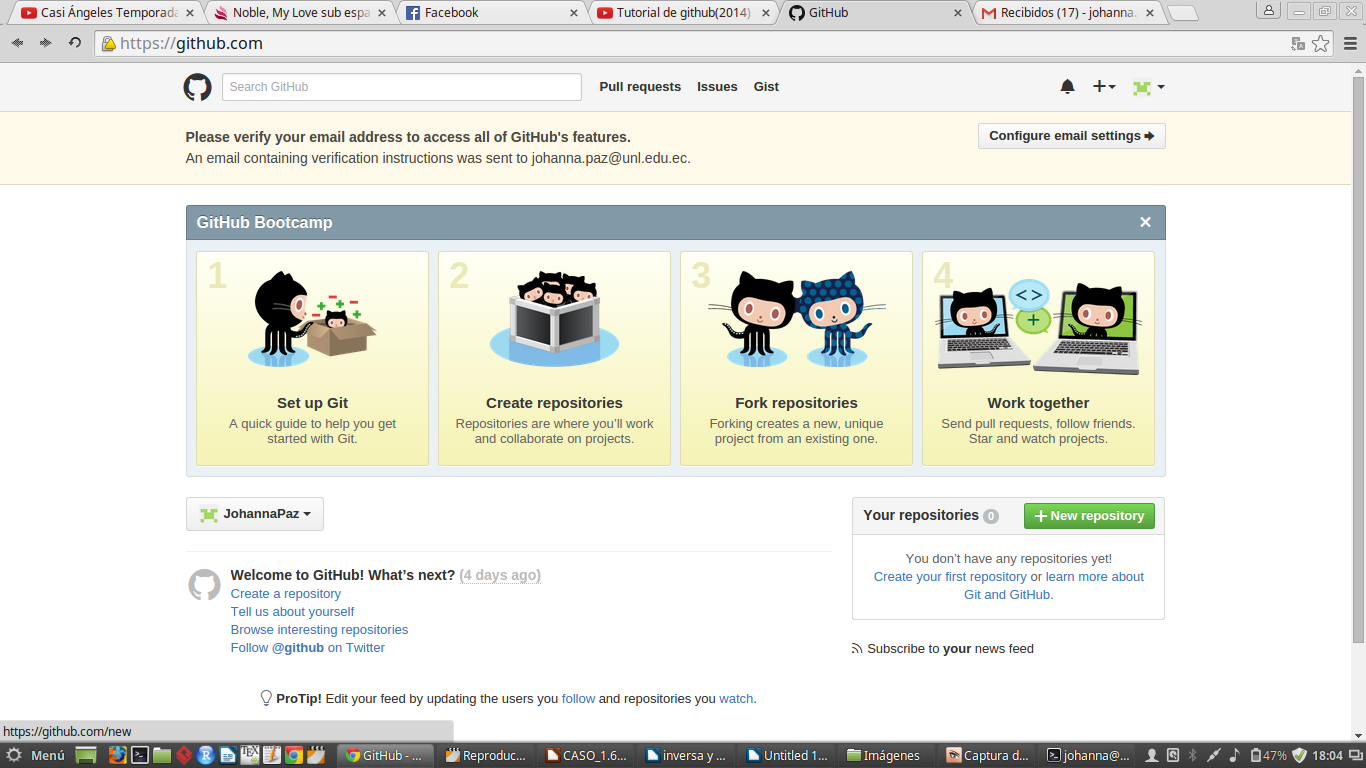
\includegraphics[width=17cm,height=9.557cm]{manual-img3.png}
\end{center}
{\sffamily
Ahora vamos \ a crear el nuevo repositorio asi:}


\bigskip



\begin{center}
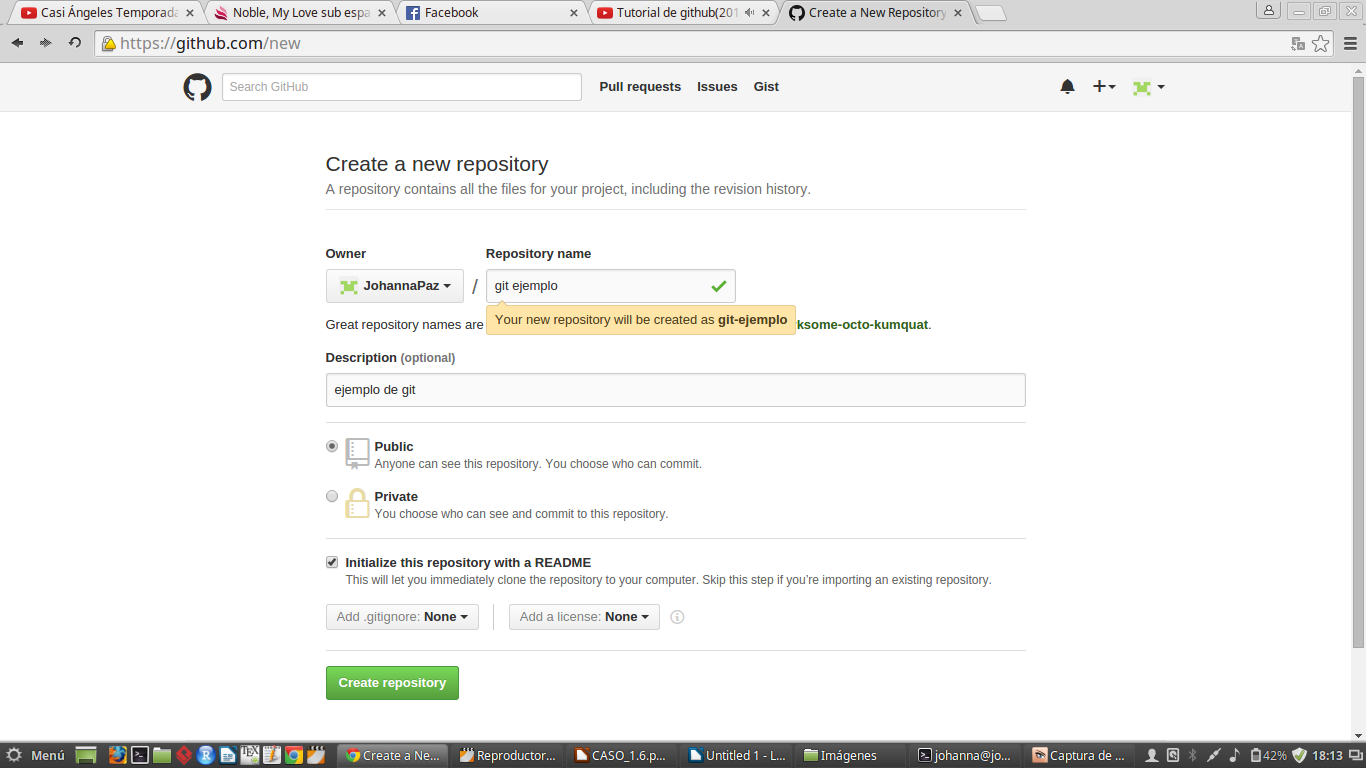
\includegraphics[width=17cm,height=9.557cm]{manual-img4.png}
\end{center}

\bigskip

{\sffamily
Veamos como quedo creado el nuevo repositorio.}

\textstyleFuentedeprrafopredeter{\textsf{\newline
git clone }}\url{https://github.com/JohannaPaz/git-ejemplo}

\begin{center}
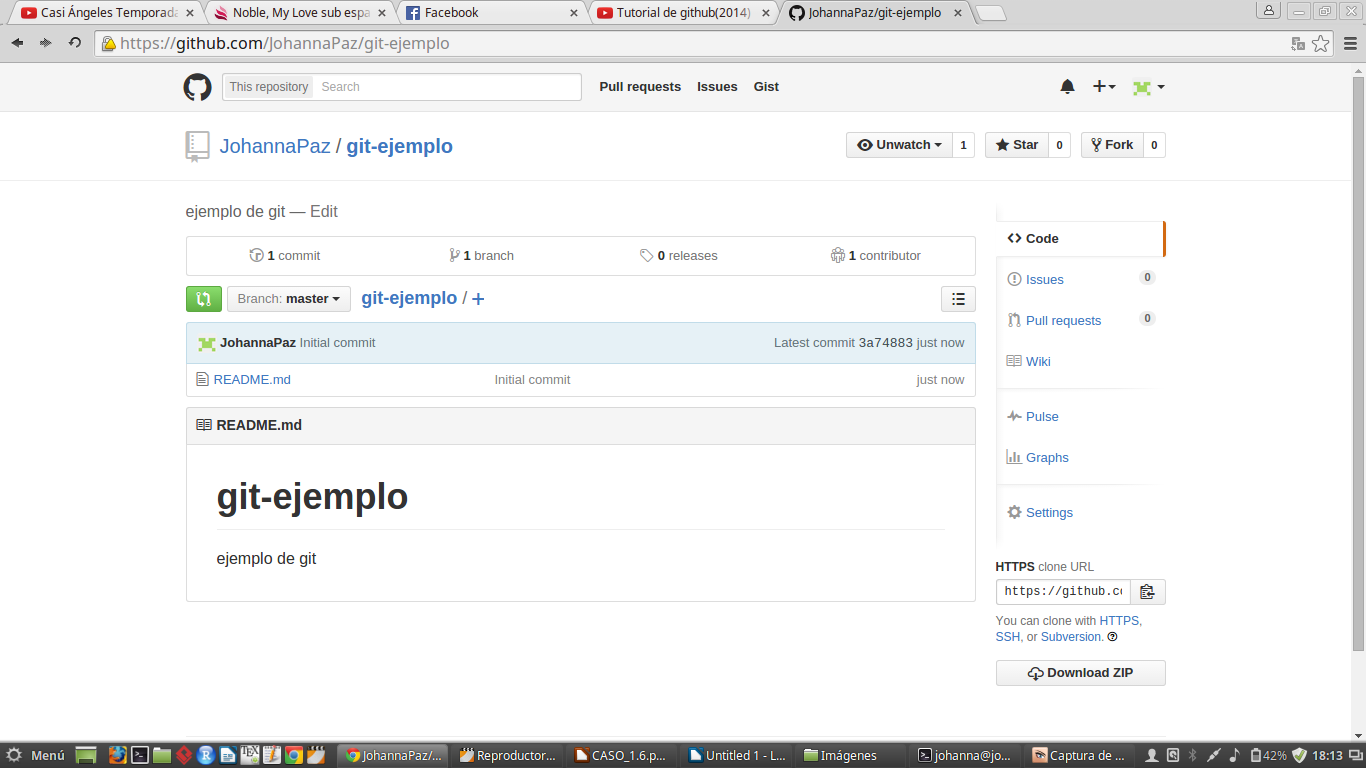
\includegraphics[width=17cm,height=9.557cm]{manual-img5.png}
\end{center}

\bigskip

\liststyleLi
\setcounter{saveenum}{\value{enumi}}
\begin{enumerate}
\setcounter{enumi}{\value{saveenum}}
\item {\sffamily
Una vez creado nuestro repositorio lo que tenemos que hacer es clonarlo.
Para \ ello tenemos que crear una carpeta en cualquier lugar yo lo
hecho as\'i, la carpeta con tiene el nombre de git proyecto}
\end{enumerate}


\begin{center}
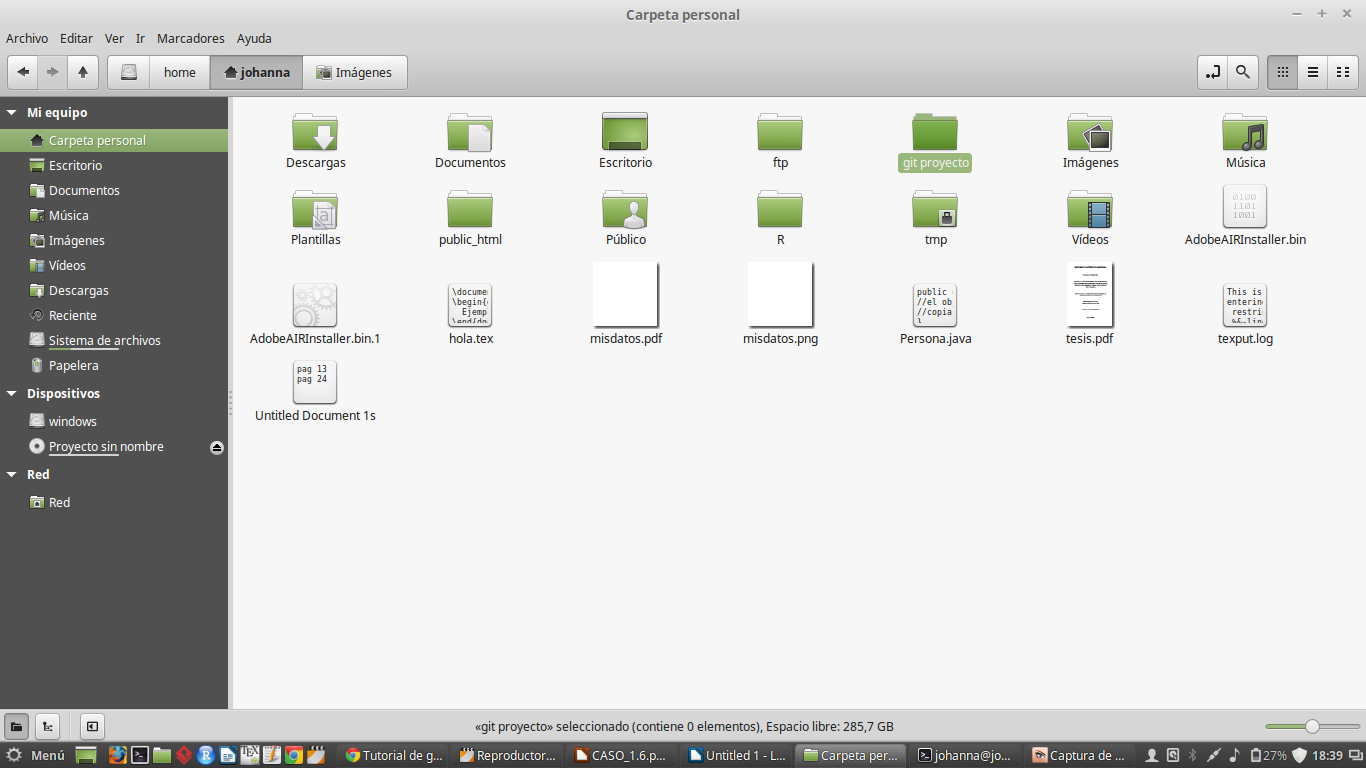
\includegraphics[width=17cm,height=9.557cm]{manual-img6.png}
\end{center}
\liststyleLi
\setcounter{saveenum}{\value{enumi}}
\begin{enumerate}
\setcounter{enumi}{\value{saveenum}}
\item {\sffamily
Ahora accedemos a la consola y escribimos los siguientes comandos para
poder clonar la carpeta.}
\end{enumerate}
{\sffamily
\ \ \ \ cd git{\textbackslash} proyecto/}

{\sffamily
\ \ \ \ ls}

{\sffamily
\ \ \ \ git clone https://github.com/JohannaPaz/git-ejemplo.git}

{\sffamily
Verificamos que se ha clonado la \ carpeta as\'i:}



\begin{center}
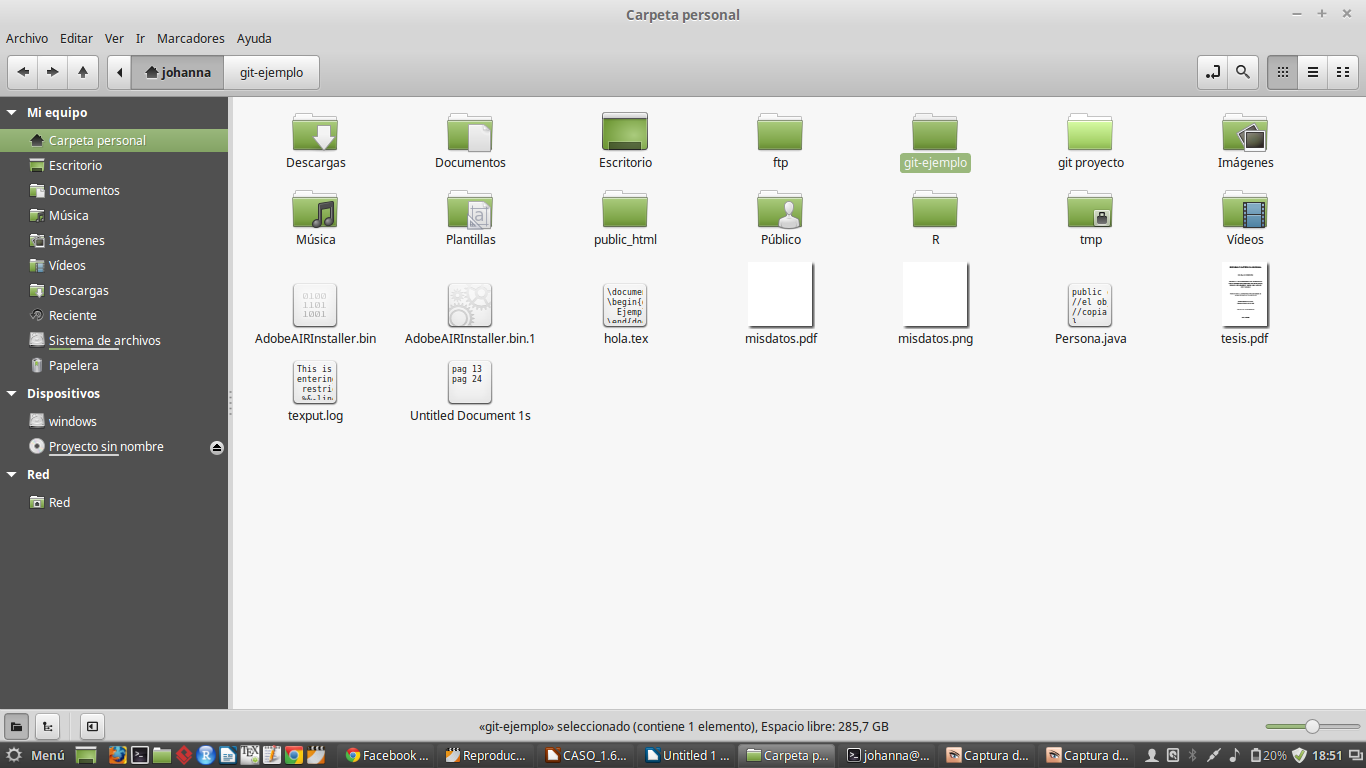
\includegraphics[width=17cm,height=9.557cm]{manual-img7.png}
\end{center}
\liststyleLi
\setcounter{saveenum}{\value{enumi}}
\begin{enumerate}
\setcounter{enumi}{\value{saveenum}}
\item {\sffamily
Instalar git gui\newline
\ \  sudo apt-get install gitk giggle git-cola git-gui gitg}
\item {\sffamily
\ Abrir el gui de git mediante el comando, para eso tenemos q estar en
la carpeta donde clonamos el git.\newline
 \ \ git gui}
\item {\sffamily
Poner el nombre del usuario en git\newline
 \ \ git config -{}-global user.name nombre\newline
 \ \ \ \ colocar email del usuario\newline
 \ \ git config -{}-global user.email email}
\item {\sffamily
git pull origin master\newline
\ \  para asegurarnos de que no exista ning\'un cambio que nosotros no
tengamos.}
\item {\sffamily
git push origin master\newline
\ \ subimos los cambios.}
\end{enumerate}

\bigskip
\end{document}
